% \begin{name}
% 	{GV biên soạn: Mai Thái Phong\\ GV phản biện: Hải Phụng}
% 	{TOÁN 10-KNTT-CS}
% \end{name}
%----------------NỘI DUNG BIÊN SOẠN
\setcounter{chapter}{3}
\chap{VECTƠ}
\setcounter{section}{6}

\section{Các khái niệm mở đầu}
%-------------------------------------------
\subsection{KIẾN THỨC TRỌNG TÂM}
\subsubsection{Khái niệm vectơ}
\begin{khung4}{}
	\begin{itemize}
		\item  \textbf{Vectơ} là một đoạn thẳng có hướng, nghĩa là, trong hai điểm mút của đoạn thẳng, đã chỉ rõ điểm đầu, điểm cuối.
		\item \textbf{Độ dài của vectơ} là khoảng cách giữa điểm đầu và điểm cuối của vectơ đó.
	\end{itemize}
\end{khung4}
\begin{note}
	\immini{
	\begin{itemize}
		\item Vectơ có điểm đầu $A$ và điểm cuối $B$ được kí hiệu là $\overrightarrow{AB}$, đọc là vectơ $AB$; vectơ còn được kí hiệu là $\overrightarrow{a}, \overrightarrow{b}, \dots$.
		\item Độ dài của vectơ $\overrightarrow{AB}, \overrightarrow{a}$ tương ứng được kí hiệu là $\left|\overrightarrow{AB}\right|$, $\left|\overrightarrow{a}\right|$.
	\end{itemize}
}{
\begin{minipage}{0.35\textwidth}
	\centering
	\begin{tikzpicture}[line join=round, line cap=round,>=stealth,
		font=\footnotesize,scale=1.2]
		\path
		(0,0) coordinate (A)
		(2,1) coordinate (B)
		($(A)!1/2!(B)$) coordinate (F);
		\draw[line width=1pt,->] (A)--(B) node[below]{$B$};
		% \draw (F) node[below=0.75cm]{Hình $4.3$};
		\fill (A) circle (1.2pt) node[below]{$A$};
	\end{tikzpicture}
	\\[1cm]
	\begin{tikzpicture}[line join=round, line cap=round,>=stealth,
		font=\footnotesize,scale=0.8]
		\draw[->] (0,0)--++(1.5,0) node[midway,above]{$\overrightarrow{a}$};
		\draw[->] (2.5,-1)--++(0.75,1.5) node[midway,right]{$\overrightarrow{b}$};
		% \draw[->] (4.25,0)--++(1,-0.25) node[midway,above]{$\overrightarrow{x}$};
		% \draw[<-] (6.25,0)--++(0.75,0.25) node[midway,below]{$\overrightarrow{y}$};
		% \draw (3.5,-1.25) node[]{Hình $4.4$};
	\end{tikzpicture}
\end{minipage}
}
\end{note}
\subsubsection{Hai vectơ cùng phương, cùng hướng, bằng nhau}
\begin{khung4}{}
	\immini{
	\begin{itemize}
		\item Đường thẳng đi qua điểm đầu và điểm cuối của một vectơ được gọi là giá của vectơ đó.
		\item Hai vectơ được gọi là cùng phương nếu chúng có giá song song hoặc trùng nhau.
	\end{itemize}
}{
\begin{tikzpicture}[line join = round, line cap=round,>=stealth,font=\footnotesize,scale=1]
	\path
	(0,0) coordinate (A)
	(5,1) coordinate (B)
	;
	\draw[dashed] (A)--(B);
	\draw[dashed] ($(A)+(0,1)$)--($(B)+(0,1)$);
	\draw[dashed] ($(A)+(0,2)$)--($(B)+(0,2)$);
	\draw[red, line width=1pt,<-] ($(A)!1/4!(B)$)--($(A)!5/6!(B)$)node[midway,above]{$\overrightarrow{d}$};
	\draw[red, line width=1pt,->] ($(A)+(0,1.11)!1/10!(B)$)--($(A)!1/2!(B)+(0,1)$)node[midway,above]{$\overrightarrow{b}$};
	\draw[red, line width=1pt,<-] ($(A)+(0,3)!2/3!(B)$)--($(A)!6/7!(B)+(0,1)$)node[midway,above]{$\overrightarrow{c}$};
	\draw[red, line width=1pt,->] ($(A)+(0,4)!1/2!(B)$)--($(A)!5/7!(B)+(0,2)$)node[midway,above]{$\overrightarrow{a}$};
\end{tikzpicture}
}
\end{khung4}
\begin{khung4}{}
	Hai vectơ cùng phương thì chúng cùng hướng hoặc ngược hướng.
\end{khung4}
\begin{khung4}{}
	Hai vectơ $\overrightarrow{a}$ và $\overrightarrow{b}$ được gọi là bằng nhau, kí hiệu $\overrightarrow{a} = \overrightarrow{b}$, nếu chúng có cùng độ dài và cùng hướng.
\end{khung4}
\begin{note}
	\immini{
	\begin{itemize}
		\item Ta cũng xét các vectơ có điểm đầu và điểm cuối trùng nhau (chẳng hạn $\overrightarrow{AA}$, $\overrightarrow{BB}$, $\overrightarrow{MM}$), gọi là các \textbf{vectơ-không}.
		\item Ta quy ước vectơ-không có độ dài bằng $0$, cùng hướng (do đó cùng phương) với mọi vectơ.
		\item Các vectơ-không có cùng độ dài và cùng hướng nên bằng nhau và được kí hiệu chung là $\overrightarrow{0}$.
		\item Với mỗi điểm $O$ và vectơ $\overrightarrow{a}$ cho trước, có duy nhất điểm $A$ sao cho $\overrightarrow{OA} = \overrightarrow{a}$.
	\end{itemize}
}{
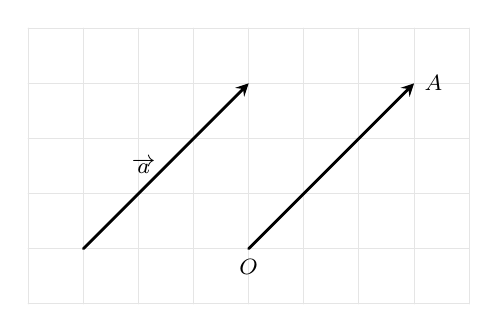
\begin{tikzpicture}[line join = round, line cap=round,>=stealth,font=\footnotesize,scale=0.7]
	\draw[opacity=0.1] (-4,-1) grid (4,4);
	\path
	(0,0) coordinate (O)
	(3,3) coordinate (A)
	;
	\draw[->,line width=1pt] (O)node[below]{$O$}--(A)node[right]{$A$};
	\draw[->,line width=1pt] (-3,0)--(0,3)node[midway,left]{$\overrightarrow{a}$};
\end{tikzpicture}
}
\end{note}
\begin{khung4}{}
	Ba điểm $A$, $B$, $C$ thẳng hàng khi và chỉ khi $\overrightarrow{AB}$, $\overrightarrow{AC}$ cùng phương.
\end{khung4}
\begin{note}
	Ta có thể dùng vectơ để biểu diễn các đại lượng như lực, vận tốc, gia tốc. Hướng của vectơ chỉ hướng của đại lượng, độ dài của vectơ thể hiện cho độ lớn của đại lượng và được lấy tỉ lệ với độ lớn của đại lượng.
\end{note}
\subsection{PHÂN LOẠI VÀ PHƯƠNG PHÁP GIẢI TOÁN}
\begin{dang}{Xác định vectơ; xác định phương và hướng của vectơ}
\end{dang}
%%=====VD1=======%%
\begin{vd}%[0H5N1-1]
	\immini{Cho tam giác $ABC$. Hãy kể tên các vectơ (khác $\overrightarrow{0}$) có điểm đầu và điểm cuối là các đỉnh của tam giác.\dongcham{3}}{
	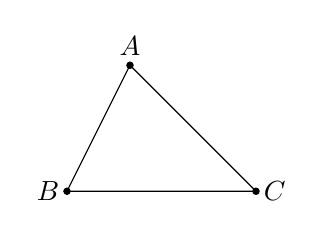
\begin{tikzpicture}[smooth,scale=0.8]
		\path
		(0,0) coordinate (B)
		(3,0) coordinate (C)
		(1,2) coordinate (A);
		\draw (A)--(B)--(C)--(A);
		\foreach \x/\g in {A/90,B/180,C/0} \draw [fill=black] (\x) circle (.05) + (\g:.3) node{$\x$};
	\end{tikzpicture}}
\loigiai{
	Các vectơ có thể là $\overrightarrow{AB}$, $\overrightarrow{BA}$, $\overrightarrow{AC}$, $\overrightarrow{CA}$, $\overrightarrow{BC}$, $\overrightarrow{CB}$.}
\end{vd}

%%=====VD2=======%%
\begin{vd}%[0H5H1-2]
	\immini{Cho hình bình hành $ABCD$ tâm $O$ như hình bên.
	\begin{enumerate}
		\item Kể tên 2 vectơ cùng phương với vectơ $\overrightarrow{OA}$.
		\item Kể tên vectơ cùng hướng, ngược hướng với vectơ $\overrightarrow{OB}$.
	\end{enumerate}
	}{
	\begin{tikzpicture}[smooth,font=\footnotesize,scale=0.6]
		\path
		(0,0) coordinate (A)
		(1,2) coordinate (B)
		(4,2) coordinate (C)
		(3,0) coordinate (D);
		\coordinate (O) at ($(C)!0.5!(A)$);
		\draw (A)--(B)--(C)--(D)--cycle (A)--(C) (B)--(D);
		\foreach \x/\g in {A/-90,B/90,C/90,D/-90,O/90} \draw [fill=black] (\x) circle (.05) + (\g:.3) node{$\x$};
	\end{tikzpicture}}
\loigiai{
	\begin{enumerate}
		\item Hai vectơ cùng phương với $\overrightarrow{OA}$ là $\overrightarrow{AC}$, $\overrightarrow{OC}$.\\
		Ngoài ra còn có $\overrightarrow{CA}$, $\overrightarrow{AO}$, $\overrightarrow{CO}$...
		\item Vectơ cùng hướng với $\overrightarrow{OB}$ là $\overrightarrow{DB}$, $\overrightarrow{DO}$;\\
		Vectơ ngược hướng với $\overrightarrow{OB}$ là $\overrightarrow{BO}$, $\overrightarrow{OD}$ và $\overrightarrow{BD}$.
	\end{enumerate}}
\end{vd} \dongcham{3}
%%=====Dạng 2=======%%
\begin{dang}{Hai vectơ bằng nhau, đối nhau}
\end{dang}
%%=====VD3=======%%
\begin{vd}%[0H5N1-3]
	\immini{Cho tam giác $ABC$. Các điểm $M$, $N$ và $K$ lần lượt là trung điểm của $AB$, $AC$ và $BC$.
	\begin{enumerate}
		\item Tìm các vectơ bằng với $\overrightarrow{AM}$.
		\item Tìm các vectơ bằng với $\overrightarrow{KN}$.
	\end{enumerate}}{
	\begin{tikzpicture}[scale=0.8, line join=round, line cap=round]
		\tkzDefPoints{0/0/A,1/2/B,4/0/C}
		\coordinate (M) at ($(A)!0.5!(B)$);
		\coordinate (N) at ($(C)!0.5!(A)$);
		\coordinate (K) at ($(B)!0.5!(C)$);
		\tkzDrawSegments(A,B B,C C,A M,N N,K M,K)
		\tkzDrawPoints[size=2,fill=black](A,B,C,M,N,K)
		\tkzLabelPoints[below, font=\footnotesize](A,N,C)
		\tkzLabelPoints[above, font=\footnotesize](B)
		\tkzLabelPoints[above left, font=\footnotesize](M)
		\tkzLabelPoints[above right, font=\footnotesize](K)
	\end{tikzpicture}}
\loigiai{
	\begin{enumerate}
		\item Vì $M$ là trung điểm của $AB$ nên vectơ bằng với $\overrightarrow{AM}$ là $\overrightarrow{MB}$.\\
		Vì $NK$ là đường trung bình của $\triangle ABC$ nên vectơ bằng với $\overrightarrow{AM}$ là $\overrightarrow{NK}$.
		\item Vì $NK$ là đường trung bình của $\triangle ABC$ nên vectơ bằng với $\overrightarrow{KN}$ là $\overrightarrow{BM}$ và $\overrightarrow{MA}$.
	\end{enumerate}
	}
\end{vd} \dongcham{4}
%%=====VD4=======%%
\begin{vd}%[0H5H1-3]
	\immini{Cho lục giác đều $ABCDEF$ tâm $O$.
	\begin{enumerate}
		\item Tìm các vectơ bằng với $\overrightarrow{EF}$.
		\item Tìm các vectơ là vectơ đối của $\overrightarrow{OB}$.
	\end{enumerate}
	\dongcham{3}}{
	\begin{tikzpicture}[scale=0.7]
		\tkzDefPoint(0,0){O}
		\tkzDefPoint(2,0){E}
		\tkzDefPointBy[rotation=center O angle 60](E) \tkzGetPoint{F}
		\tkzDefPointBy[rotation=center O angle 120](E) \tkzGetPoint{A}
		\tkzDefPointBy[rotation=center O angle 180](E) \tkzGetPoint{B}
		\tkzDefPointBy[rotation=center O angle 240](E) \tkzGetPoint{C}
		\tkzDefPointBy[rotation=center O angle 300](E) \tkzGetPoint{D}
		\tkzDrawPoints[size=2,fill=black](A,B,C,D,E,F,O)
		\tkzDrawSegments(A,B B,C C,D D,E E,F F,A A,D F,C B,E)
		\draw (A) node[above] {$A$} (B) node[left] {$B$} (C) node[below] {$C$} (D) node[below] {$D$} (E) node[right] {$E$} (F) node[above] {$F$} (O) node[below left] {$O$};
	\end{tikzpicture}
	}
\loigiai{
	\begin{enumerate}
		\item Các vectơ bằng với $\overrightarrow{EF}$ là $\overrightarrow{CB}$, $\overrightarrow{OA}$, $\overrightarrow{DO}$.
		\item Các vectơ đối của $\overrightarrow{OB}$ là $\overrightarrow{AF}$, $\overrightarrow{OE}$, $\overrightarrow{CD}$.
	\end{enumerate}
	}
\end{vd}
%%=====Dạng 3=======%%
\begin{dang}{Độ dài vectơ}
	Độ dài của $\overrightarrow{AB}$ là độ dài đoạn thẳng $AB$. Khi tính toán, ta có thể chú ý đến định lý Pythagore và các tỉ số lượng giác của góc nhọn trong tam giác vuông.
\end{dang}
%%=====VD5=======%%
\begin{vd}%[0H5H1-5]
	\immini{Cho hình vuông $ABCD$ tâm $O$, cạnh bằng $2$.
	\begin{enumerate}
		\item Tính độ dài của các vectơ $\overrightarrow{AB}$, $\overrightarrow{AC}$ và $\overrightarrow{AO}$.
		\item Gọi $I$ là trung điểm của $BC$. Tính độ dài của $\overrightarrow{AI}$.
	\end{enumerate}
	}{
	\begin{tikzpicture}[smooth,font=\footnotesize,scale=1]
		\path
		(0,0) coordinate (A)
		(2,0) coordinate (B)
		(2,2) coordinate (C)
		(0,2) coordinate (D);
		\coordinate (O) at ($(B)!0.5!(D)$);
		\draw (A)--(B)--(C)--(D)--(A) (A)--(C) (B)--(D);
		\foreach \x/\g in {A/-90,B/-90,C/90,D/90,O/0} \draw [fill=black] (\x) circle (.045) + (\g:.3) node{$\x$};
	\end{tikzpicture}
	}
\loigiai{
	\begin{center}
		\begin{tikzpicture}[smooth,font=\footnotesize,scale=1]
			\path
			(0,0) coordinate (A)
			(2,0) coordinate (B)
			(2,2) coordinate (C)
			(0,2) coordinate (D);
			\coordinate (I) at ($(B)!0.5!(C)$);
			\coordinate (O) at ($(B)!0.5!(D)$);
			\draw (A)--(B)--(C)--(D)--(A) (A)--(C) (B)--(D) (A)--(I);
			\foreach \x/\g in {A/-90,B/-90,C/90,D/90,O/0,I/0} \draw [fill=black] (\x) circle (.045) + (\g:.3) node{$\x$};
		\end{tikzpicture}
	\end{center}
	\begin{enumerate}
		\item Độ dài của $\overrightarrow{AB}$ là $\left|\overrightarrow{AB}\right|=AB=2$.\\
		Độ dài của $\overrightarrow{AC}$ là $\left|\overrightarrow{AC}\right|=AC=AB\cdot\sqrt{2}=2\sqrt{2}$.\\
		Độ dài của $\overrightarrow{AO}$ là $\left|\overrightarrow{AO}\right|=AO=\dfrac{AB\cdot\sqrt{2}}{2}=\sqrt{2}$.
		\item
		Vì $I$ là trung điểm của $BC$ nên $IB=\dfrac{BC}{2}=1$.\\
		Vì $\triangle ABI$ vuông tại $B$ nên $AI=\sqrt{AB^2+BI^2}=\sqrt{2^2+1^2}=\sqrt{5}$.\\
		Độ dài của $\overrightarrow{AI}$ là $\left|\overrightarrow{AI}\right|=AI=\sqrt{5}$.
	\end{enumerate}
	}
\end{vd}
\dongcham{6}
%%=====VD6=======%%
\begin{vd}%[0H5V1-5]
	Cho tam giác $ABC$ đều, cạnh bằng $3$. Gọi $H$ là trung điểm của $BC$ và $G$ là trọng tâm tam giác $ABC$.
	\begin{enumerate}
		\item Hãy tính độ dài của  $\overrightarrow{AH}$.
		\item Hãy tính độ dài của  $\overrightarrow{GB}$.
	\end{enumerate}
\loigiai{
	\begin{center}
		\begin{tikzpicture}[scale=1.2,font=\footnotesize]
			\path (0,0) coordinate (B)--++(0:3) coordinate (C) --++(120:3) coordinate (A);
			\coordinate (H) at ($(B)!0.5!(C)$);
			\coordinate (G) at ($(A)!2/3!(H)$);
			% Vẽ tam giác và các đoạn thẳng cần thiết
			\draw (A)--(B)--(C)--cycle;
			\draw (A)--(H);
			\draw (A)--(G);
			% Vẽ điểm
			\foreach \point/\pos in {A/above,B/below,C/below,H/below right,G/right}
			\filldraw (\point) circle (1pt) node[\pos]{$\point$};
		\end{tikzpicture}
	\end{center}
	\begin{enumerate}
		\item Vì $\triangle ABC$ đều có cạnh $3$ nên $AB=BC=3$. Suy ra $BH=\dfrac{BC}{2}=\dfrac{3}{2}$.\\
		Mặt khác $AH$ cũng là đường cao của $\triangle ABC$ nên $AH \perp BC$.\\
		Xét $\triangle AHB$ vuông tại $H$ có $AH=\sqrt{AB^2-HB^2}=\sqrt{3^2-\left(\dfrac{3}{2}\right)^2}=\dfrac{3\sqrt{3}}{2}$.\\
		Vậy $\left|\overrightarrow{AH}\right|=\dfrac{3\sqrt{3}}{2}$.
		\item Vì $G$ là trọng tâm của $\triangle ABC$ nên $GH=\dfrac{1}{3}AH=\dfrac{\sqrt{3}}{2}$.\\
		Xét $\triangle GHB$ vuông tại $H$ có $GB=\sqrt{GH^2+HB^2}=\sqrt{\left(\dfrac{\sqrt{3}}{2}\right)^2+\left(\dfrac{3}{2}\right)^2}=\sqrt{3}$.\\
		Vậy $\left|\overrightarrow{GB}\right|=GB=\sqrt{3}$.
	\end{enumerate}
	}
\end{vd}
\dongcham{6}
%-------------------------------------------
\subsection{BÀI TẬP RÈN LUYỆN}
%-------------Trắc nghiệm nhiều lựa chọn
\caulc
\setcounter{ex}{0}
\Opensolutionfile{ans}[ans/ans-c4b7-lc]
%%=======Câu 1=======%%
\begin{ex}%[0H5N1-1]
	Vectơ có điểm đầu $D$, điểm cuối $E$ được kí hiệu là
	\choice
	{$\overrightarrow{ED}$}
	{\True $\overrightarrow{DE}$}
	{$\overline{DE}$}
	{$\left| \overrightarrow{DE}\right| $}
\loigiai{
	Vectơ có điểm đầu $D$, điểm cuối $E$ được kí hiệu là $\overrightarrow{DE}$.
	}
\end{ex}
%%=======Câu 2=======%%
\begin{ex}%[0H5N1-2]
	Cho hình bình hành $ABCD$. Có bao nhiêu vectơ khác vectơ-không cùng phương với $\overrightarrow{AB}$ có điểm đầu và cuối là các đỉnh của hình bình hành?
	\choice
	{\True $3$}
	{$4$}
	{$6$}
	{$5$}
\loigiai{
	Các vectơ khác vectơ-không cùng phương vectơ $\overrightarrow{AB}$ là  $\overrightarrow{BA}$, $\overrightarrow{CD}$ và $\overrightarrow{DC}$.
	}
\end{ex}
%%=======Câu 3=======%%
\begin{ex} %[0H5N1-2]
	Cho ba điểm $M, N, P$ thẳng hàng, trong đó $N$ nằm giữa hai điểm $M$ và $P$. Khi đó cặp vectơ nào sau đây cùng hướng?
	\choice
	{$\vec{MP}$ và $\vec{PN}$}
	{$\vec{MN}$ và $\vec{PN}$}
	{$\vec{NP}$ và $\vec{NM}$}
	{\True $\vec{MN}$ và $\vec{MP}$}
\loigiai{
	\begin{center}
		\begin{tikzpicture}[line join=round, line cap=round,>=stealth,font=\footnotesize,scale=1]
			\draw (0,0) coordinate (M) --++(0:2) coordinate (N)--++(0:3) coordinate(P);
			\foreach\x/\g in {M/90, N/90, P/90}{
			\draw[fill=black] (\x) circle (1pt)+(\g:0.3) node {$\x$};
			};
		\end{tikzpicture}
	\end{center}
	$\vec{MN}$ và $\vec{MP}$ cùng hướng.
	}
\end{ex}
%%=======Câu 4=======%%
\begin{ex}%[0H5N1-3]
	\immini{
	Cho lục giác đều $ABCDEF$ tâm $O$. Hãy tìm các vectơ khác vectơ-không có điểm đầu, điểm cuối là đỉnh của lục giác và tâm $O$ sao cho bằng với $\overrightarrow{AB}$.
	\choice
	{\True $\overrightarrow{FO}$, $\overrightarrow{OC}$, $\overrightarrow{ED}$}
	{$\overrightarrow{BO}$, $\overrightarrow{OC}$, $\overrightarrow{ED}$}
	{$\overrightarrow{FO}$, $\overrightarrow{AC}$, $\overrightarrow{ED}$}
	{$\overrightarrow{FO}$, $\overrightarrow{OC}$, $\overrightarrow{FD}$}
	}
	{
	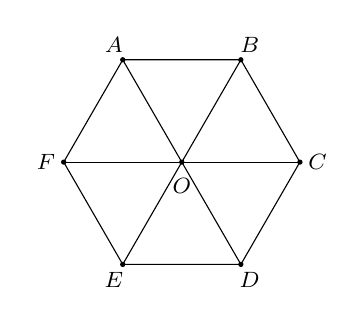
\begin{tikzpicture}[scale=0.75, font=\footnotesize, line join=round, line cap=round, >=stealth]
		\def\r{2}
		\path (0,0) coordinate (O);
		\foreach\x/\y in {A/120,B/60,C/0,D/-60,E/-120,F/180}
		{\path (\y:\r) coordinate (\x);
		\draw (O)--(\x);
		\draw[fill=black] (\x) circle (1pt)+(\y:0.3) node{$\x$};
		}
		\draw (A)--(B)--(C)--(D)--(E)--(F)--(A);
		\draw[fill=black] (O) circle (1pt)+(-90:0.4) node{$O$};
	\end{tikzpicture}
	}
\loigiai{
	Các vectơ khác vectơ-không bằng với $\overrightarrow{AB}$ là các vectơ $\overrightarrow{FO}$, $\overrightarrow{OC}$, $\overrightarrow{ED}$.
	}
\end{ex}
%%=======Câu 5=======%%
\begin{ex}%[0H5N1-5]
	Mệnh đề nào sau đây \textbf{sai}?
	\choice
	{$|\overrightarrow{A B}|=|\overrightarrow{B A}|$}
	{Vectơ $\overrightarrow{0}$ cùng hướng với mọi vectơ}
	{\True $\overrightarrow{A A}=0$}
	{Vectơ $\overrightarrow{0}$ cùng phương với mọi vectơ}
\loigiai{
	Ta có $\overrightarrow{A A}=\overrightarrow{0}$ nên mệnh đề $\overrightarrow{A A}=0$ sai.
	}
\end{ex}
%%=======Câu 6=======%%
\begin{ex}%[0H5H1-5]
	Cho hình chữ nhật $ABCD$ có $AB=a$, $AD=2a$. Tính $\left|\overrightarrow{AC}\right|$.
	\choice
	{$3a$}
	{\True $\sqrt{5}a$}
	{$\sqrt{2}a$}
	{$2a$}
\loigiai{
	\begin{center}
		\begin{tikzpicture}[scale=0.8, font=\footnotesize,line join=round, line cap=round, >=stealth,rotate=90]
			\def\a{2} %%chiều dài
			\def\b{4} %%chiều rộng
			\path
			(0,0) coordinate (A)
			(\a,0) coordinate (B)
			(0,-\b) coordinate (D)
			($(B)+(D)-(A)$) coordinate (C)
			($(B)!1/2!(C)$) coordinate (M)
			($(C)!1/3!(D)$) coordinate (N)
			;
			\draw (A)--(B) node[midway,left]{$a$}
			(A)--(D) node[midway,below]{$2a$}
			(D)--(C)--(B)
			;
			\foreach \x/\y/\z in {A/B/C, D/A/B, D/C/B, C/D/A}
			{pic[draw,angle eccentricity=1.8,angle radius=2mm]{right angle = \x--\y--\z}}
			;
			\foreach \i/\g in {A/90,B/90,C/-90,D/-90}
			\fill[black] (\i) circle(1pt)+(\g:3mm)node[scale=1]{$\i$};
		\end{tikzpicture}
	\end{center}
	Ta có $\left|\overrightarrow{AC}\right|=AC$.\\
	Sử dụng định lý Pythagore ta giải được $AC=\sqrt{5}a$.
	}
\end{ex}
%%=======Câu 7=======%%
\begin{ex}%[0H5H1-2]
	\immini[thm]{Cho hình bình hành $ABCD$ tâm $O$. Trên hình vẽ, số vectơ (khác $\overrightarrow{0}$, khác $\overrightarrow{AC}$) cùng phương với vectơ $\overrightarrow{AC}$ là
	\choice
	{$2$}
	{$3$}
	{$4$}
	{\True $5$}}{
	\begin{tikzpicture}[scale=1,line join=round,line cap=round, >=stealth]
		\def\a{4}
		\def\g{60}
		\path
		(0,0) coordinate (A)
		(A)++(0:\a) coordinate (B)
		(B)++(\g:\a/2) coordinate (C)
		($(A)+(C)-(B)$) coordinate (D)
		(intersection of A--C and B--D) coordinate (O)
		;
		\draw
		(A)--(B)--(C)--(D)--cycle
		(A)--(C) (B)--(D)
		;
		\foreach \x/\g in {A/-135, B/-45, C/45, D/135, O/-90}{
		\draw[fill=black] (\x) circle (0.045) +(\g:0.3) node {$\x$};
		};
	\end{tikzpicture}}
\loigiai{Các vectơ (khác $\overrightarrow{0}$, khác $\overrightarrow{AC}$) cùng phương với $\overrightarrow{AC}$ là: $\overrightarrow{AO}$, $\overrightarrow{OA}$, $\overrightarrow{CO}$, $\overrightarrow{OC}$, $\overrightarrow{CA}$.}
\end{ex}
%%=======Câu 8=======%%
\begin{ex}%[0H5N1-3]
	Gọi $M$ là trung điểm của đoạn thẳng $AB$. Khẳng định nào sau đây là khẳng định đúng?
	\choice
	{\True $\overrightarrow{AB}$ và $\overrightarrow{AM}$ cùng phương}
	{$\overrightarrow{MA}=\overrightarrow{MB}$}
	{$\left|\overrightarrow{AB}\right|=\left|\overrightarrow{MB}\right|$}
	{$\overrightarrow{AB}$ và $\overrightarrow{MB}$ ngược hướng}
\loigiai{
	\centerline{
	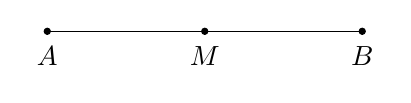
\begin{tikzpicture}[scale=1, line join=round, line cap=round, >=stealth]
		%% Khai bao diem
		\path
		(0,0) coordinate (A)
		(2,0) coordinate (M)
		(4,0) coordinate (B)
		;
		\draw (A)--(B);
		%% vẽ điểm
		\foreach \x/\g in {A/-90,M/-90,B/-90}
		\draw[fill=black] (\x) circle (.039)+(\g:.31)
		node{$\x$};
	\end{tikzpicture}}	\\
	Ta có $\overrightarrow{AB}$ và $\overrightarrow{AM}$ cùng phương.}
\end{ex}
%%=======Câu 9=======%%
\begin{ex}%[0H5V1-3]
	Cho tam giác $ABC$. Có bao nhiêu vectơ khác $\overrightarrow{0}$ có điểm đầu và điểm cuối là các đỉnh của tam giác $ABC$?
	\choice
	{$3$}
	{\True $6$}
	{$9$}
	{$8$}
\loigiai{
	Các vectơ khác vectơ $\overrightarrow{0}$ thỏa mãn là $\overrightarrow{AB}$, $\overrightarrow{AC}$, $\overrightarrow{BC}$, $\overrightarrow{BA}$, $\overrightarrow{CA}$, $\overrightarrow{CB}$.
	}
\end{ex}
%%=======Câu 10=======%%
\begin{ex}%[0H5H1-3]
	Cho hình chữ nhật $ABCD$ có tâm là $I$. Khẳng định nào sau đây là đúng?
	\choice
	{$\overrightarrow{IC}=\overrightarrow{DI}$}
	{\True $\overrightarrow{AI}=\overrightarrow{IC}$}
	{$\overrightarrow{BI}=\overrightarrow{DI}$}
	{$\overrightarrow{IA}=\overrightarrow{BI}$}
\loigiai{
	\immini{Do $I$ là tâm của hình chữ nhật $ABCD$ nên $I$ là trung điểm của $AC$.\\Vậy ta có $\overrightarrow{AI}=\overrightarrow{IC}$.}
	{\begin{tikzpicture}[scale=1, line join=round, line cap=round]
	\def\d{4}
	\def\r{2.5}
	\path
	(0,0) coordinate (D)
	(0:\d) coordinate (C)
	(90:\r) coordinate (A)
	($(A)+(C)-(D)$) coordinate (B)
	(intersection of A--C and B--D) coordinate (I)
	;
	\draw (A)--(B)--(C)--(D)--(A)--(C) (B)--(D);
	\foreach \x/\g in {A/135,B/45,C/-45,D/-135,I/-90}
	\draw[fill=black] (\x) circle (.04)+(\g:.31)
	node{$\x$};
	\end{tikzpicture}}
	}
\end{ex}
%%=======Câu 12=======%%
\begin{ex}%[0H5N1-3]
	Cho bốn điểm phân biệt $A$, $B$, $C$, $D$ thỏa mãn $\overrightarrow{AB}=\overrightarrow{DC}$. Khẳng định nào sau đây là khẳng định \textbf{sai}?
	\choice
	{$AB=CD$}
	{$\overrightarrow{AB}$ và $\overrightarrow{DC}$ là hai vectơ cùng hướng}
	{$AC$ và $BD$ nhận cùng một điểm làm trung điểm}
	{\True $ABCD$ là hình bình hành}
\loigiai{
	$ABCD$ là hình bình hành khi và chỉ khi bốn điểm $A$, $B$, $C$, $D$ không thẳng hàng và $\overrightarrow{AB}=\overrightarrow{DC}$.}
\end{ex}
%%=======Câu 13=======%%
\begin{ex}%[0H5N1-2]
	Cho tam giác $ABC$ có $M$, $N$ lần lượt là trung điểm của hai cạnh $AB$ và $AC$. Khẳng định nào sau đây là khẳng định đúng?
	\choice
	{$\overrightarrow{MN}$ và $\overrightarrow{AC}$ cùng phương}
	{\True $\overrightarrow{MN}$ và $\overrightarrow{BC}$ cùng phương}
	{$\overrightarrow{MN}$ và $\overrightarrow{AB}$ cùng phương}
	{$\overrightarrow{MN}$ và $\overrightarrow{BN}$ cùng phương}
\loigiai{
	\immini{
	Ta có $MN$ là đường trung bình của tam giác $ABC$ nên $MN\parallel BC$. Do đó hai vectơ $\overrightarrow{MN}$ và $\overrightarrow{BC}$ cùng phương.
	}
	{
	\begin{tikzpicture}[scale=1,line join=round, line cap=round,>=stealth]
		\path
		(0,0) coordinate (B)
		(0:4) coordinate (C)
		(70:3) coordinate (A)
		($(A)!0.5!(B)$) coordinate (M)
		($(A)!0.5!(C)$) coordinate (N)
		;
		\draw (A)--(B)--(C)--(A) (M)--(N);
		\foreach \x/\g in {A/90,B/-135,C/-45,M/160,N/20}
		\draw[fill=black] (\x) circle (.04)+(\g:.31)
		node{$\x$};
	\end{tikzpicture}
	}
	}
\end{ex}
\Closesolutionfile{ans}
\indapan{6}{ans/ans-c4b7-lc}
%---------------------Trắc nghiệm đúng sai
\cauds
\setcounter{ex}{0}
\Opensolutionfile{ans}[ans/ans-c4b7-ds]
\begin{ex}%[0H5N1-3]
	Gọi ${K}$ là trung điểm của đoạn thẳng ${PQ}$.
	\choiceTF
	{\True $\overrightarrow{QP}$ cùng phương với $\overrightarrow{QK}$}
	{$\overrightarrow{KP}=\overrightarrow{KQ}$}
	{$\left|\overrightarrow{QP}\right|=\left|\overrightarrow{QK}\right|$}
	{$\overrightarrow{QP}$ ngược hướng với $\overrightarrow{QK}$}
\loigiai{
	\centerline{
	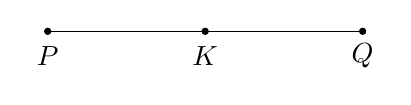
\begin{tikzpicture}[scale=1, line join=round, line cap=round, >=stealth]
		%% Khai bao diem
		\path
		(0,0) coordinate (P)
		(2,0) coordinate (K)
		(4,0) coordinate (Q)
		;
		\draw (P)--(Q);
		%% vẽ điểm
		\foreach \x/\g in {P/-90,K/-90,Q/-90}
		\draw[fill=black] (\x) circle (.039)+(\g:.31)
		node{$\x$};
	\end{tikzpicture}}
	\begin{itemchoice}
		\itemch Vì $P$, $K$, $Q$ thẳng hàng ($K$ là trung điểm của $PQ$) nên $\overrightarrow{QP}$ cùng phương với $\overrightarrow{QK}$.
		\itemch Vì $\overrightarrow{KP}$ ngược hướng với $\overrightarrow{KQ}$ nên hai vectơ không thể bằng nhau.
		\itemch $\left|\overrightarrow{QK}\right|=\dfrac{1}{2}\left|\overrightarrow{QP}\right|$, nên không bằng nhau.
		\itemch $\overrightarrow{QP}$ và $\overrightarrow{QK}$ cùng hướng.
	\end{itemchoice}
	}
\end{ex}
\begin{ex}%[0H5N1-3]
	\immini[thm]{Cho hình bình hành ${ABCD}$ tâm $O$.
	\choiceTF
	{\True $\overrightarrow{DA}$ và $\overrightarrow{CB}$ là cùng hướng }
	{$\overrightarrow{OA}=\overrightarrow{OC}$}
	{\True $\left|\overrightarrow{OB}\right|=\left|\overrightarrow{OD}\right|$}
	{$\left|\overrightarrow{AC}\right|=\left|\overrightarrow{BD}\right|$}
	}{\begin{tikzpicture}[scale=1,line join=round,line cap=round, >=stealth]
	\def\a{4}
	\def\g{60}
	\path
	(0,0) coordinate (A)
	(A)++(0:\a) coordinate (B)
	(B)++(\g:\a/2) coordinate (C)
	($(A)+(C)-(B)$) coordinate (D)
	(intersection of A--C and B--D) coordinate (O)
	;
	\draw
	(A)--(B)--(C)--(D)--cycle
	(A)--(C) (B)--(D)
	;
	\foreach \x/\g in {A/135, B/-45, C/60, D/150, O/-95}{
	\draw[fill=black] (\x) circle (0.045) +(\g:0.3) node {$\x$};
	};
	\end{tikzpicture}}
\loigiai{
	\begin{itemchoice}
		\itemch Vì $ABCD$ là hình bình hành nên $DA \parallel CB$ và $DA=CB$.\\
		Suy ra $\overrightarrow{DA}$ cùng hướng với $\overrightarrow{CB}$ và $\left|\overrightarrow{DA}\right|=\left|\overrightarrow{CB}\right|$.\\
		Vậy $\overrightarrow{DA}=\overrightarrow{CB}$.
		\itemch Vì $O$ là trung điểm của $AC$ nên $\overrightarrow{OA}$ và $\overrightarrow{OC}$ ngược hướng nhau.
		\itemch $O$ là trung điểm của $BD$ nên $\left|\overrightarrow{OB}\right|=\left|\overrightarrow{OD}\right|$.
		\itemch Vì $ABCD$ không là hình chữ nhật nên độ dài $AC$ và $BD$ khác nhau.
	\end{itemchoice}
	}
\end{ex}
\begin{ex}%[0H5N1-5]
	\immini[thm]{Cho hình vuông ${ABCD}$ cạnh bằng $a$, $I$ là điểm trên cạnh $BC$ thỏa $CI=\dfrac{1}{2}IB$.
	\choiceTF
	{\True $\overrightarrow{DA}$ và $\overrightarrow{BC}$ là ngược hướng }
	{ $\overrightarrow{AC}=\overrightarrow{BD}$ }
	{$\left|\overrightarrow{AC}\right|=2a$}
	{\True $\left|\overrightarrow{AI}\right|=\dfrac{\sqrt{13}a}{3}$}}{\begin{tikzpicture}[scale=1, line join=round, line cap=round]
	\def\d{3}
	\def\r{3}
	\path
	(0,0) coordinate (D)
	(0:\d) coordinate (C)
	(90:\r) coordinate (A)
	($(A)+(C)-(D)$) coordinate (B)
	($(C)!1/3!(B)$) coordinate (I)
	;
	\draw (A)--(B)--(C)--(D)--(A)--(I);
	\foreach \x/\g in {A/135,B/45,C/-45,D/-135,I/0}
	\draw[fill=black] (\x) circle (.04)+(\g:.31)
	node{$\x$};
	\end{tikzpicture}}
\loigiai{	\begin{itemchoice}
	\itemch Vì $ABCD$ là hình bình hành nên $DA \parallel BC$. Suy ra $\overrightarrow{DA}$ cùng phương với $\overrightarrow{BC}$\\
	Xét về chiều, ta có được $\overrightarrow{DA}$ ngược hướng với $\overrightarrow{BC}$.
	\itemch Hai vectơ $\overrightarrow{AC}$ và $\overrightarrow{BD}$ không cùng phương nên hai vectơ không bằng nhau.
	\itemch Độ dài đường chéo $AC$ của hình vuông là $a\sqrt{2}$. Suy ra $\left|\overrightarrow{AC}\right|=a\sqrt{2}$.
	\itemch  Đặt $CI=x$ $(x>0)$, khi đó $IB=2x$.\\
	Ta có $CI+IB=CB \Leftrightarrow 3x=a \Leftrightarrow x=\dfrac{a}{3}$.\\
	Suy ra $CI=\dfrac{a}{3}$ và $IB=\dfrac{2a}{3}$.\\
	Xét $AIB$ vuông tại $B$, áp dụng định lí Pythagore có
	\[AB^2+BI^2=AI^2 \Rightarrow AI=\sqrt{AB^2+BI^2} =\dfrac{a\sqrt{13}}{3}.		\]
	\end{itemchoice}}
\end{ex}
\begin{ex}%[0H5N1-5]
	Cho hình chữ nhật $ABCD$ có $O$ là giao điểm của hai đường chéo và $AB=a$, $BC=3a$.
	\choiceTF
	{\True $\left|\overrightarrow{DC}\right|=a$}
	{$\left|\overrightarrow{AD}\right|=4a$}
	{\True $\left|\overrightarrow{BD}\right|=\sqrt{10}a$}
	{\True $\left|\overrightarrow{OB}\right|=\dfrac{\sqrt{10}a}{2}$}
\loigiai{
	\immini{\begin{itemchoice}
	\itemch Vì$ABCD$ là hình chữ nhật nên nên $CD=AB$.\\
	Suy ra $\left|\overrightarrow{DC}\right|=CD=AB=a$.
	\itemch Vì$ABCD$ là hình chữ nhật nên nên $AD=BC$.\\
	Suy ra $\left|\overrightarrow{AD}\right|=AD=BC=3a$.
	\itemch Đường chéo $BD=\sqrt{AB^2+AD^2}=\sqrt{a^2+(3a)^2}=\sqrt{10}a$.\\
	Suy ra $\left|\overrightarrow{BD}\right|=BD=a\sqrt{10}$.
	\itemch $O$ là trung điểm đường chéo $BD$ nên $OB=\dfrac{1}{2}BD=\dfrac{a\sqrt{10}}{2}$.\\
	Suy ra $\left|\overrightarrow{OB}\right|=OB=\dfrac{a\sqrt{10}}{2}$.
	\end{itemchoice}
	}{\begin{tikzpicture}[scale=1, line join=round, line cap=round]
	\def\d{4}
	\def\r{2.5}
	\path
	(0,0) coordinate (D)
	(0:\d) coordinate (C)
	(90:\r) coordinate (A)
	($(A)+(C)-(D)$) coordinate (B)
	(intersection of A--C and B--D) coordinate (O)
	;
	\draw (A)--(B)--(C)--(D)--(A)--(C) (B)--(D);
	\foreach \x/\g in {A/135,B/45,C/-45,D/-135,O/-90}
	\draw[fill=black] (\x) circle (.04)+(\g:.31)
	node{$\x$};
	\end{tikzpicture}}
	}
\end{ex}
\Closesolutionfile{ans}
\indapan{3}{ans/ans-c4b7-ds}
%---------------Trắc nghiệm trả lời ngắn
\caukq
\setcounter{ex}{0}
\Opensolutionfile{ans}[ans/ans-c4b7-kq]
%-----Câu 1
\begin{ex}%[0H5H1-2]
	Cho các vectơ như hình vẽ. Có bao nhiêu cặp vectơ cùng phương xuất hiện trong hình?
	\shortans[oly]{$8$}
	\begin{center}
		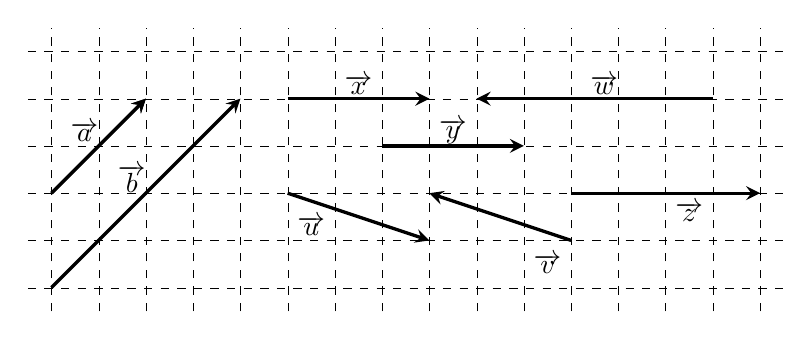
\begin{tikzpicture}[line width=1.2,>=stealth,scale=0.6]
			\draw[step=1,ultra thin,dashed](-0.5,-0.5)grid(15.5,5.5);
			\draw[->](0,2)--(2,4);
			\draw[->](0,0)--(4,4);
			\draw[->](5,4)--(8,4);
			\draw[->](5,2)--(8,1);
			\draw[->](7,3)--(10,3);
			\draw[->](0,2)--(2,4);
			\draw[->](14,4)--(9,4);
			\draw[->](11,2)--(15,2);
			\draw[->](11,1)--(8,2);
			\node at (0.7,3.3) {$\overrightarrow{a}$};
			\node at (1.7,2.3) {$\overrightarrow{b}$};
			\node at (5.5,1.3) {$\overrightarrow{u}$};
			\node at (10.5,0.5) {$\overrightarrow{v}$};
			\node at (13.5,1.6) {$\overrightarrow{z}$};
			\node at (6.5,4.3) {$\overrightarrow{x}$};
			\node at (8.5,3.3) {$\overrightarrow{y}$};
			\node at (11.7,4.3) {$\overrightarrow{w}$};
		\end{tikzpicture}
	\end{center}
\loigiai{
	Có $8$ cặp vectơ cùng phương xuất hiện trong hình gồm: $\overrightarrow{a}$ và $\overrightarrow{b}$, $\overrightarrow{x}$ và $\overrightarrow{y}$, $\overrightarrow{x}$ và $\overrightarrow{z}$, $\overrightarrow{x}$ và $\overrightarrow{w}$, $\overrightarrow{y}$ và $\overrightarrow{z}$, $\overrightarrow{y}$ và $\overrightarrow{w}$, $\overrightarrow{z}$ và $\overrightarrow{w}$, $\overrightarrow{u}$ và $\overrightarrow{v}$.}
\end{ex}
\begin{ex}%[0H5N1-5]
	Cho hình vuông $ABCD$ có độ dài cạnh bằng $3$ cm. Tính độ dài của $\overrightarrow{AC}$. (kết quả làm tròn đến hai chữ số thập phân)
	\shortans[oly]{$4{,}24$}
\loigiai{
	\immini{
	$\left|\overrightarrow{AC}\right|=AC=\sqrt{AB^2+BC^2}=\sqrt{3^2+3^2}=3\sqrt{2} \approx 4{,}24$ cm.
	}{
	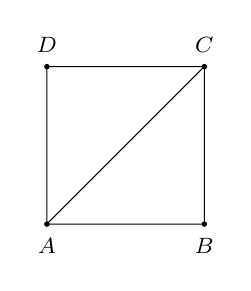
\begin{tikzpicture}[scale=1, font=\footnotesize, line join=round, line cap=round,>=stealth]
		\draw (0,0) rectangle (2,2) (0,0)--(2,2);
		\foreach\i/\j/\goc/\diem in{0/0/-90/A,2/0/-90/B,2/2/90/C,0/2/90/D}
		\fill(\i,\j) circle(1.0pt) node[shift={(\goc:8pt)}]{$\diem$};
	\end{tikzpicture}
	}
	}
\end{ex}
\begin{ex}%[0H5N1-5]
	\immini{
	Cho hình chữ nhật $ABCD$ có cạnh $AB=3$, $BC=4$. Độ dài của $\overrightarrow{DB}$ bằng bao nhiêu?	
	}{
	\begin{tikzpicture}[scale=0.8, font=\footnotesize, line join=round, line cap=round, >=stealth]
		\path	(0,0) coordinate (A)++(0:3) coordinate (D)
		($(A)+(-90:2)$) coordinate (B)
		($(B)+(D)-(A)$) coordinate (C)
		;
		\draw (A)--(B)--(C)--(D)--(A);
		\foreach \x/\g in {A/130,D/60,C/-30,B/-150}  \fill (\x) circle (1pt)+(\g:.3)node[scale=0.8]{$\x$};
	\end{tikzpicture}
	}
	\shortans[oly]{$5$}
\loigiai{
	Áp dụng định lí Pythagore cho tam giác vuông $ABC$ ta có
	\[ AC=\sqrt{AB^2+BC^2}=\sqrt{3^2+4^2}=5. \]
	Vì $ABCD$ là hình chữ nhật nên $\left|\overrightarrow{DB}\right|=\left|\overrightarrow{AC}\right|=AC=5$.
	}
\end{ex}
\begin{ex}%[0H5N1-5]
	Cho tam giác $ABC$ đều cạnh bằng $1$, trọng tâm $G$. Độ dài của $\overrightarrow{AG}$ bằng bao nhiêu? (kết quả làm tròn đến hai chữ số thập phân)
	\shortans[oly]{$0{,}58$}
\loigiai{
	\immini
	{
	Gọi $I$ là trung điểm của $BC \Rightarrow AI=\dfrac{\sqrt{3}}{2}$.\\
	Ta có $AG=\dfrac{2}{3}AI=\dfrac{2}{3} \cdot \dfrac{\sqrt{3}}{2}=\dfrac{\sqrt{3}}{3} \Rightarrow \left|\overrightarrow{AG}\right|=\dfrac{\sqrt{3}}{3}\approx 0,58$.
	}
	{
	\begin{tikzpicture}[>=stealth,line cap=round,line join=round,scale=.6,font=\footnotesize]
		\tkzDefPoints{-2/-3/B,4/-3/C}
		\tkzDefPointBy[rotation=center B angle 60](C)    \tkzGetPoint{A}
		\coordinate (I) at ($(C)!0.5!(B)$);
		\tkzCentroid(A,B,C)    \tkzGetPoint{G}
		\tkzDrawPolygon(A,B,C)
		\tkzDrawPoints[fill=black](A,B,C,I,G)
		\tkzDrawSegments(G,I)
		\draw[blue,->](A)--(G);
		\tkzLabelPoints[left](G,B)
		\tkzLabelPoints[above](A)
		\tkzLabelPoints[below](I)
		\tkzLabelPoints[right](C)
	\end{tikzpicture}
	}
	}
\end{ex}
\begin{ex}%[0H5V1-5]
	Cho hình thoi $ABCD$ cạnh $a$ và $\widehat{BAD}=60^\circ$. Tìm độ dài vectơ $\overrightarrow{AC}$.
	\shortans{$a\sqrt{3}$}
	\loigiai
	{
	\begin{center}
		\begin{tikzpicture}[scale=1, font=\footnotesize, line join=round, line cap=round, >=stealth]
			\path
			(0,0) coordinate (A) node[below left]{$A$}
			(3,0) coordinate (D) node[below right]{$D$}
			(60:3) coordinate (B) node[above left]{$B$}
			($(B)+(D)-(A)$) coordinate (C) node[above right]{$C$}
			;
			\draw
			(A)--(B)--(C)--(D)--cycle
			;
			\draw[->]
			(A)--(C)
			;
			\foreach \x in {A,B,C,D}
			\draw[fill=black] (\x) circle (1pt);
		\end{tikzpicture}
	\end{center}
	Xét tam giác $ADC$, do $ABCD$ là hình thoi nên
	\begin{align*}
		\widehat{ADC}=180^\circ-\widehat{BAD}=120^\circ\quad\text{và}\quad AD=CD=a.
	\end{align*}
	Áp dụng định lý Côsin, ta được
	\begin{align*}
		AC^2=AD^2+DC^2-2\cdot AD\cdot DC\cdot \cos \widehat{ADC}=a^2+a^2-2a^2\cos 120^\circ=3a^2
	\end{align*}
	Vậy
	\begin{align*}
		\left|\overrightarrow{AC}\right|=AC=a\sqrt{3}.
	\end{align*}
	}
\end{ex}
\begin{ex}%[0H5N1-5]
	Cho tam giác $ABC$ đều có cạnh bằng $8$. Gọi $G$ là trọng tâm tam giác $ABC$ và $I$ là trung điểm của $AG$. Độ dài của $\overrightarrow{AI}$ (làm tròn kết quả đến hàng phần trăm) bằng bao nhiêu?
	\shortans[oly]{$2{,}31$}
\loigiai{
	\immini{
	Gọi $M$ là trung điểm của $BC$. Ta có
	\[\begin{array}{l} {\left|\overrightarrow{AG}\right|=AG=\dfrac{2}{3} AM=\dfrac{2}{3} \sqrt{AB^2-BM^2}=\dfrac{2}{3} \sqrt{8^2-\dfrac{8^2}{4}}=\dfrac{8\sqrt{3}}{3}} \\ {\left|\overrightarrow{AI}\right|=AI=\dfrac{AG}{2}=\dfrac{4\sqrt{3}}{3} \approx 2{,}31} \end{array}
	\]
	}{
	\begin{tikzpicture}[scale=1, font=\footnotesize, line join=round, line cap=round, >=stealth]
		\path	(0,0) coordinate (B)++(0:3) coordinate (C)
		($(B)+(60:3)$) coordinate (A)
		($(B)!1/2!(C)$) coordinate (M)
		($(A)!2/3!(M)$) coordinate (G)
		($(A)!1/2!(G)$) coordinate (I)
		;
		\draw (A)--(B)--(C)--(A)--(M);
		\foreach \x/\g in {A/90,B/-150,C/-30,I/0,G/0,M/-90}  \fill (\x) circle (1pt)+(\g:.3)node[scale=1]{$\x$};
	\end{tikzpicture}
	}
	}
\end{ex}
\Closesolutionfile{ans}
\indapan{4}{ans/ans-c4b7-kq}
%------------------Tự luận
\TL
\setcounter{bt}{0}
\begin{bt}%[0H5H1-2]
	\immini{
	Quan sát hình bên và gọi tên các vectơ:
	\begin{enumerate}[a)]
		\item Cùng phương với vectơ $\overrightarrow{x}$.
		\item Cùng hướng với vectơ $\overrightarrow{a}$.
		\item Ngược hướng với vectơ $\overrightarrow{u}$.
	\end{enumerate}
	}{
	\begin{tikzpicture}[scale=.6, font=\footnotesize, line join=round, line cap=round,>={Stealth[length=2mm]}]
		\def\xmin{0} \def\xmax{13}
		\def\ymin{0} \def\ymax{7}
		\draw[color=gray!50,dashed] (\xmin,\ymin) grid (\xmax,\ymax);
		\draw[->] (1,6)--(2,4);
		\draw (1.5,5) node [left] {$\overrightarrow{a}$};
		\draw[->] (3,6)--(4.5,3);
		\draw (3,4) node [above right] {$\overrightarrow{b}$};
		\draw[->] (6,6)--(11,6);
		\draw(8.5,6) node [above] {$\overrightarrow{z}$};
		\draw[->] (6,3)--(8,5);
		\draw(7,4) node [left] {$\overrightarrow{u}$};
		\draw[->] (10,5)--(8,3);
		\draw(9,4) node [left] {$\overrightarrow{v}$};
		\draw[->] (8,2)--(10,2);
		\draw(9,2) node [above] {$\overrightarrow{y}$};
		\draw[->] (2,1)--(5,1);
		\draw(3.5,1) node [above] {$\overrightarrow{x}$};
		\draw[->] (12,1)--(6,1);
		\draw(9,1) node [above] {$\overrightarrow{w}$};
		%	\draw (6.5,-.5) node{Hình 8};
		\fill (1,6) circle (2pt) (3,6)circle (2pt) (6,6)circle (2pt) (6,3)circle (2pt) (10,5)circle (2pt) (2,1)circle (2pt) (12,1)circle (2pt);
	\end{tikzpicture}
	}
\loigiai{
	\begin{enumerate}[a)]
		\item Cùng phương với vectơ $\overrightarrow{x}$ là $\overrightarrow{y}$, $\overrightarrow{z}$, $\overrightarrow{w}$.
		\item Cùng hướng với vectơ $\overrightarrow{a}$ là $\overrightarrow{b}$.
		\item Ngược hướng với vectơ $\overrightarrow{u}$ là $\overrightarrow{v}$.
	\end{enumerate}
	}
\end{bt}
\begin{bt}%[0H5H1-2]
	Hãy chỉ ra các cặp vectơ cùng hướng, ngược hướng, bằng nhau trong hình dưới đây.
	\begin{center}
		\begin{tikzpicture}[scale=.8, font=\footnotesize, line join=round, line cap=round,>={Stealth[length=2mm]}]
			\def\xmin{0} \def\xmax{10}
			\def\ymin{0} \def\ymax{6}
			\draw[color=gray!50,dashed] (\xmin,\ymin) grid (\xmax,\ymax);
			\draw[->] (2,5)--(1,3);
			\draw (1,5) node [below right] {$\overrightarrow{a}$};
			\draw[->] (3,5)--(1,1);
			\draw (3,3) node [above left] {$\overrightarrow{b}$};
			\draw[->] (5,5)--(8,5);
			\draw(6,5) node [above right] {$\overrightarrow{y}$};
			\draw[->] (6,4)--(8,3);
			\draw(7,4) node [below right] {$\overrightarrow{v}$};
			\draw[->] (9,2)--(5,2);
			\draw(8,2) node [above left] {$\overrightarrow{x}$};
			\draw[->] (3,2)--(5,1);
			\draw(4,2) node [below right] {$\overrightarrow{u}$};
			%	\draw (6.5,-.5) node{Hình 17};
			\fill (2,5) circle (2pt) (3,5)circle (2pt) (5,5)circle (2pt) (6,4)circle (2pt) (9,2)circle (2pt) (3,2)circle (2pt);
		\end{tikzpicture}
	\end{center}
\loigiai{
	Ta có
	\begin{itemize}
		\item Các cặp vectơ cùng hướng là $\overrightarrow{a}$ và $ \overrightarrow{b}$, $\overrightarrow{u}$ và $\overrightarrow{v}$.
		\item Cặp vectơ ngược hướng là $\overrightarrow{x}$ và $\overrightarrow{y}$
		\item Cặp vectơ bằng nhau là $\overrightarrow{u}$ và $\overrightarrow{v}$.
	\end{itemize}
	}
\end{bt}
\begin{bt}%[0H5H1-2]
	\immini{
	Cho hình thang $ ABCD$ có hai cạnh đáy là $ AB$ và $ DC$ (hình bên). Điểm $ M$ nằm trên đoạn $ DC$.
	\begin{enumerate}
		\item Gọi tên các vectơ cùng hướng với vectơ $ \overrightarrow{AB}$.
		\item Gọi tên các vectơ ngược hướng với vectơ $ \overrightarrow{DM}$.
	\end{enumerate}}
	{
	\begin{tikzpicture}[scale=.7, font=\footnotesize, line join=round, line cap=round,>={Stealth[length=2mm]}]
		\draw (0,0) node [below left] {$ D$}--(6,0) node [below right] {$ C$}--(4,3) node [above] {$ B$}--(1,3) node [above] {$ A$}--cycle (1.5,0) node [below] {$ M$};
		\fill (0,0) circle (2pt) (6,0) circle (2pt) (4,3) circle (2pt) (1,3) circle (2pt) (1.5,0) circle (2pt);
		%	\draw (2.5,-.5) node{Hình 15};
	\end{tikzpicture}
	}
\loigiai{
	\begin{enumerate}
		\item Các vectơ cùng hướng với vectơ $ \overrightarrow{AB}$ là $ \overrightarrow{DM}$, $ \overrightarrow{MC}$, $ \overrightarrow{DC}$.
		\item Các vectơ ngược hướng với vectơ $ \overrightarrow{DM}$ là $ \overrightarrow{MD}$, $ \overrightarrow{CM}$, $ \overrightarrow{CD}$, $ \overrightarrow{BA}$.
	\end{enumerate}
	}
\end{bt}
\begin{bt}%[0H5H1-1]
	\immini{
	Cho hình vuông $ ABCD$ có tâm $ O$ và có cạnh bằng $ a$ (hình bên).
	\begin{enumerate}
		\item Tìm trong hình hai vectơ bằng nhau và có độ dài bằng $ \dfrac{a\sqrt{2}}{2}$.
		\item Tìm trong hình hai vectơ đối nhau và có độ dài bằng $ a\sqrt{2}$.
	\end{enumerate}}
	{
	\begin{tikzpicture}[scale=0.7, font=\footnotesize, line join=round, line cap=round, >=stealth]
		\def\dc{4} % cạnh BC
		\def\da{4} % cạnh BA
		\def\h{4} % đường cao
		\def\gocD{90} % góc B của đáy
		\coordinate[label=below:$D$] (D) at (0,0);
		\coordinate[label=above:$A$] (A) at (\gocD:\da);
		\coordinate[label=below:$C$] (C) at (\dc,0);
		\coordinate[label=above:$B$] (B) at ($(A)+(C)-(D)$);
		\draw (A)--(D)--(C)--(B)--cycle (A)--(C) (B)--(D);
		\foreach \diem in {A,B,C,D}	\fill (\diem)circle(1.5pt);
		\coordinate[label=below:$O$] (O) at ($(A)!.5!(C)$);
		\coordinate[label=left:$a$] (I) at ($(A)!.5!(D)$);
	\end{tikzpicture}
	}
\loigiai{
	\begin{enumerate}
		\item Ta có
		\begin{itemize}
			\item $ \overrightarrow{AO}=\overrightarrow{OC}$ và $ \left|\overrightarrow{AO}\right|=\left|\overrightarrow{OC} \right|=\dfrac{a\sqrt{2}}{2}$,
			\item $ \overrightarrow{OA}=\overrightarrow{CO}$ và $ \left|\overrightarrow{OA}\right|=\left|\overrightarrow{CO} \right|=\dfrac{a\sqrt{2}}{2}$,
			\item $ \overrightarrow{BO}=\overrightarrow{OD}$ và $ \left|\overrightarrow{BO}\right|=\left|\overrightarrow{OD} \right|=\dfrac{a\sqrt{2}}{2}$,
			\item $ \overrightarrow{OB}=\overrightarrow{DO}$ và $ \left|\overrightarrow{OB}\right|=\left|\overrightarrow{DO} \right|=\dfrac{a\sqrt{2}}{2}$.
		\end{itemize}
		\item Ta có
		\begin{itemize}
			\item $ \overrightarrow{AC}=-\overrightarrow{CA}$ và $ \left|\overrightarrow{AC}\right|=\left|\overrightarrow{CA} \right|=a\sqrt{2}$,
			\item$ \overrightarrow{BD}=-\overrightarrow{DB}$ và $ \left|\overrightarrow{BD}\right|=\left|\overrightarrow{DB} \right|=a\sqrt{2}$.
		\end{itemize}
	\end{enumerate}
	}
\end{bt}
\begin{bt}%[0H5H1-3]
	Cho tứ giác $ ABCD$. Chứng minh rằng tứ giác đó là hình bình hành khi và chỉ khi $ \overrightarrow{AB}=\overrightarrow{DC}$.
\loigiai{
	Ta có $ ABCD$ là hình bình hành $\Leftrightarrow \heva{&AB\parallel DC\\&AB=DC\\&\overrightarrow{AB} \text{ cùng hướng với }\overrightarrow{DC}} \Leftrightarrow \overrightarrow{AB}=\overrightarrow{DC}$.
	}
\end{bt}
\begin{bt}%[0H5H1-5]
	\immini{Cho hình vuông $ABCD$ có cạnh bằng $\dfrac{\sqrt{2}}{2}$, hai đường chéo cắt nhau tại $O$. Tìm độ dài của các vectơ $\overrightarrow{CA}$, $\overrightarrow{BD}$, $\overrightarrow{OA}$, $\overrightarrow{AO}$.}
	{
	\begin{tikzpicture}[scale=0.7, font=\footnotesize, line join=round, line cap=round, >=stealth]
		\def\dc{4} % cạnh BC
		\def\da{4} % cạnh BA
		\def\h{4} % đường cao
		\def\gocD{90} % góc B của đáy
		\coordinate[label=below:$D$] (D) at (0,0);
		\coordinate[label=above:$A$] (A) at (\gocD:\da);
		\coordinate[label=below:$C$] (C) at (\dc,0);
		\coordinate[label=above:$B$] (B) at ($(A)+(C)-(D)$);
		\draw (A)--(D)--(C)--(B)--cycle (A)--(C) (B)--(D);
		\foreach \diem in {A,B,C,D}	\fill (\diem)circle(1.5pt);
		\coordinate[label=right:$O$] (O) at ($(A)!.5!(C)$);
		\coordinate[label=left:$\dfrac{\sqrt{2}}{2}$] (I) at ($(A)!.5!(D)$);
	\end{tikzpicture}
	}
\loigiai{
	Ta có: $CA=1$, $BD=1$, $AO=\dfrac{1}{2}$.\\
	Suy ra $\left|\overrightarrow{CA} \right|=1$, $\left|\overrightarrow{BD} \right|=1$, $\left|\overrightarrow{OA} \right|= \left|\overrightarrow{AO} \right|=\dfrac{1}{2}$.
	}
\end{bt}
\Closesolutionfile{ans}